% TODO replace links each year
\newcommand{\ulmMoodleLink}{https://moodle.uni-ulm.de/course/view.php?id=37352}
\newcommand{\ulmCalendarLink}{https://moodle.uni-ulm.de/calendar/view.php?view=upcoming&course=37352}
\newcommand{\ulmMoodle}{\href{\ulmMoodleLink}{Moodle}}

\subsection{Who}

\begin{frame}{\myframetitle}
	\begin{mycolumns}[animation=none]
		\begin{example}{Who Are You?}
			\begin{itemize}
				\item a \emph{Master student} (or a \emph{Bachelor student})
				\item looking for an \emph{elective subject} \deutsch{Wahlpflicht}
				\item enrolled in \emph{Informatik}, \emph{Medieninformatik}, \emph{Software Engineering}, \ldots
				\item interested in
				\begin{itemize}
					\item \emph{learning} about the basic principles of systematically managing software variability
					\item \emph{experimenting} with novel software engineering methods and tools
					\item getting in touch with current \emph{research} on software product lines
				\end{itemize}
			\end{itemize}
		\end{example}
	\mynextcolumn
	\end{mycolumns}
\end{frame}

\begin{frame}{\myframetitle}
	\begin{mycolumns}[animation=none]
		\begin{note}{Who Are We?}
			\centering
			\href{https://www.uni-ulm.de/en/in/sp/team/thuem/}{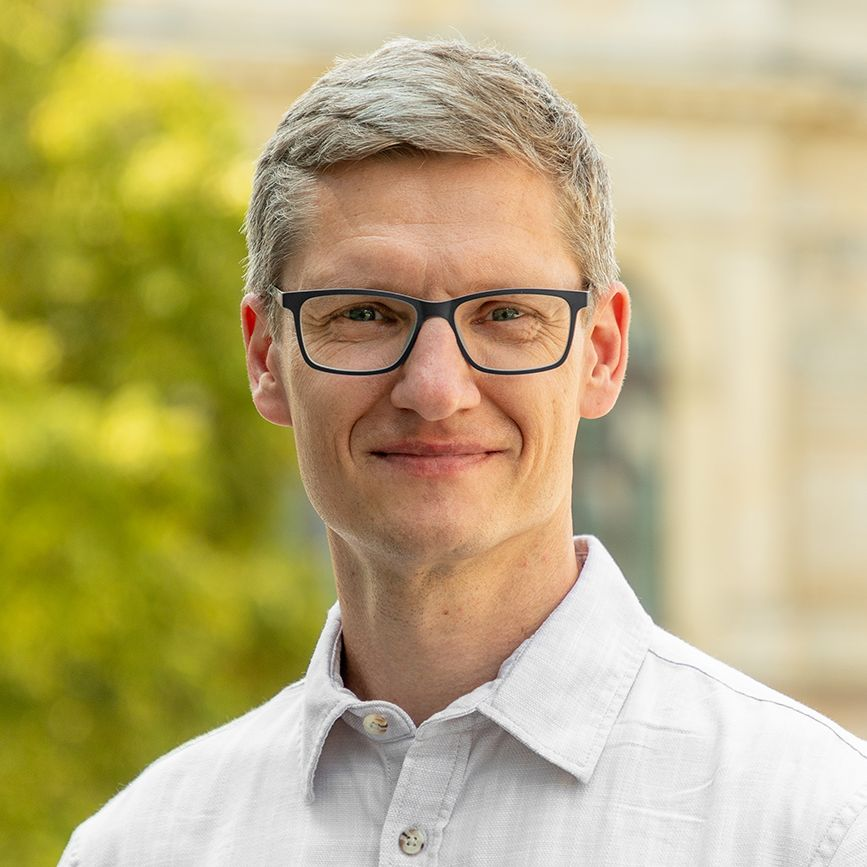
\includegraphics[height=40mm]{thomas-thuem}}\\[.5ex]
			\href{https://www.uni-ulm.de/en/in/sp/team/thuem/}{\emph{Thomas Thüm}}\\[.5ex]
			\small professor for software engineering\\[.5ex]
			FeatureIDE team leader
		\end{note}
	\mynextcolumn
		\begin{note}{Who Are We?}
			\centering
			\href{https://www.uni-ulm.de/en/in/sp/team/chico-sundermann/}{
\includegraphics[height=40mm]{chico-sundermann}}\\[.5ex]
			\href{https://www.uni-ulm.de/en/in/sp/team/chico-sundermann/}{\emph{Chico Sundermann}}\\[.5ex]
			\small PhD student in feature-model analysis\\[.5ex]
			FeatureIDE core developer
		\end{note}
	\end{mycolumns}
\end{frame}

\subsection{Where and When}

\begin{frame}{\myframetitle}
	\myframeicon{\fancyqr[image={\pic[width=10mm]{moodle-calendar}}]{https://moodle.uni-ulm.de/calendar/view.php?view=upcoming&course=37352}}
	\begin{mycolumns}
		\begin{definition}{Lecture}
			\begin{itemize}
				\item typically once per week
				\begin{itemize}
					\item exception: this week :)
					\item on \emph{Thursday}, 12:15--13:45
					\item in room O27/123
					\item next lecture April 20th
					\item see calendar on \ulmMoodle
				\end{itemize}
				\item usually held by Thomas
				\item \emph{slides} are available on \ulmMoodle
				\item \emph{videos} planned
				\item \emph{guest lecture} planned
			\end{itemize}
		\end{definition}
	\mynextcolumn
		\begin{example}{Exercise}
			\begin{itemize}
				\item typically once per week
				\begin{itemize}
					\item on \emph{Tuesday}, 90 minutes in 10:00-12:00?
					\item in room O28/H21
					\item starts on April 25th
				\end{itemize}
				\item usually held by Chico
				\item exercise sheets are available on \ulmMoodle
				\begin{itemize}
					\item \emph{theoretical tasks}
					\item \emph{practical tasks}
				\end{itemize}
			\end{itemize}
		\end{example}
	\end{mycolumns}
\end{frame}

%\subsection{Practical Tasks}

% master's theses, projects, seminars, dissertations, \ldots


\subsection{Taking the Exam, and Beyond}

\begin{frame}{\myframetitle}
	\begin{mycolumns}
		\begin{definition}{Exam}
			\begin{itemize}
				\item oral exam ($\approx 20$ minutes)
				\item 3--4 exam days during lecture-free period
				\item FAQ at the end of each lecture
			\end{itemize}
		\end{definition}
		\begin{definition}{Exam Eligibility \deutsch{Prüfungszulassung}}
			\begin{itemize}
				\item pass all 5 practical tasks $\rightarrow$ eligible for exam
				\item develop your own software product lines
				\item scope of topic is your choice
				\item submit on GitLab
			\end{itemize}
		\end{definition}
		\begin{definition}{Grade Improvement \deutsch{Notenverbesserung}}
			$\geq 7$ points for active participation in exercise, lecture, and \ulmMoodle
		\end{definition}
	\mynextcolumn
		\begin{note}{How Does the Exercise Work?}
			\begin{itemize}
				\item Prepare all tasks you want to discuss at home
				\item Recommendation: use teams to split tasks
				\item \emph{You} prepare the exercise, we moderate!
			\end{itemize}
		\end{note}

		~

		\begin{note}{Further Studies}
			\begin{itemize}
				\item \emph{SE and individual projects}
				\item \emph{seminars}
				\item \emph{bachelor's, master's, and PhD Theses}
			\end{itemize}
			\ldots{} contact us!
		\end{note}
	\end{mycolumns}
\end{frame}